\documentclass[11pt,compress,t,notes=noshow, xcolor=table]{beamer}
\usepackage[]{graphicx}\usepackage[]{color}
% maxwidth is the original width if it is less than linewidth
% otherwise use linewidth (to make sure the graphics do not exceed the margin)
\makeatletter
\def\maxwidth{ %
  \ifdim\Gin@nat@width>\linewidth
    \linewidth
  \else
    \Gin@nat@width
  \fi
}
\makeatother

\definecolor{fgcolor}{rgb}{0.345, 0.345, 0.345}
\newcommand{\hlnum}[1]{\textcolor[rgb]{0.686,0.059,0.569}{#1}}%
\newcommand{\hlstr}[1]{\textcolor[rgb]{0.192,0.494,0.8}{#1}}%
\newcommand{\hlcom}[1]{\textcolor[rgb]{0.678,0.584,0.686}{\textit{#1}}}%
\newcommand{\hlopt}[1]{\textcolor[rgb]{0,0,0}{#1}}%
\newcommand{\hlstd}[1]{\textcolor[rgb]{0.345,0.345,0.345}{#1}}%
\newcommand{\hlkwa}[1]{\textcolor[rgb]{0.161,0.373,0.58}{\textbf{#1}}}%
\newcommand{\hlkwb}[1]{\textcolor[rgb]{0.69,0.353,0.396}{#1}}%
\newcommand{\hlkwc}[1]{\textcolor[rgb]{0.333,0.667,0.333}{#1}}%
\newcommand{\hlkwd}[1]{\textcolor[rgb]{0.737,0.353,0.396}{\textbf{#1}}}%
\let\hlipl\hlkwb

\usepackage{framed}
\makeatletter
\newenvironment{kframe}{%
 \def\at@end@of@kframe{}%
 \ifinner\ifhmode%
  \def\at@end@of@kframe{\end{minipage}}%
  \begin{minipage}{\columnwidth}%
 \fi\fi%
 \def\FrameCommand##1{\hskip\@totalleftmargin \hskip-\fboxsep
 \colorbox{shadecolor}{##1}\hskip-\fboxsep
     % There is no \\@totalrightmargin, so:
     \hskip-\linewidth \hskip-\@totalleftmargin \hskip\columnwidth}%
 \MakeFramed {\advance\hsize-\width
   \@totalleftmargin\z@ \linewidth\hsize
   \@setminipage}}%
 {\par\unskip\endMakeFramed%
 \at@end@of@kframe}
\makeatother

\definecolor{shadecolor}{rgb}{.97, .97, .97}
\definecolor{messagecolor}{rgb}{0, 0, 0}
\definecolor{warningcolor}{rgb}{1, 0, 1}
\definecolor{errorcolor}{rgb}{1, 0, 0}
\newenvironment{knitrout}{}{} % an empty environment to be redefined in TeX

\usepackage{alltt}
\newcommand{\SweaveOpts}[1]{}  % do not interfere with LaTeX
\newcommand{\SweaveInput}[1]{} % because they are not real TeX commands
\newcommand{\Sexpr}[1]{}       % will only be parsed by R



\usepackage[english]{babel}
\usepackage[utf8]{inputenc}

\usepackage{dsfont}
\usepackage{verbatim}
\usepackage{amsmath}
\usepackage{amsfonts}
\usepackage{bm}
\usepackage{csquotes}
\usepackage{multirow}
\usepackage{longtable}
\usepackage{booktabs}
\usepackage{enumerate}
\usepackage[absolute,overlay]{textpos}
\usepackage{psfrag}
\usepackage{algorithm}
\usepackage{algpseudocode}
\usepackage{eqnarray}
\usepackage{arydshln}
\usepackage{tabularx}
\usepackage{placeins}
\usepackage{tikz}
\usepackage{setspace}
\usepackage{colortbl}
\usepackage{mathtools}
\usepackage{wrapfig}
\usepackage{bm}
\usetikzlibrary{shapes,arrows,automata,positioning,calc,chains,trees, shadows}
\tikzset{
  %Define standard arrow tip
  >=stealth',
  %Define style for boxes
  punkt/.style={
    rectangle,
    rounded corners,
    draw=black, very thick,
    text width=6.5em,
    minimum height=2em,
    text centered},
  % Define arrow style
  pil/.style={
    ->,
    thick,
    shorten <=2pt,
    shorten >=2pt,}
}
\usepackage{subfig}


% Defines macros and environments
\input{../../style/common.tex}
% \input{common.tex}

%\usetheme{lmu-lecture}
\usepackage{../../style/lmu-lecture}

%\usetheme{lmu-lecture}
\newcommand{\titlefigure}{figure_man/crossvalidation.png}
\newcommand{\learninggoals}{
\item Understand how resampling techniques extend the idea of simple train-test splits
\item Understand the ideas of cross-validation, bootstrap and subsampling
\item Understand what pessimistic bias means}
\usepackage{../../style/lmu-lecture}

\let\code=\texttt
\let\proglang=\textsf

\setkeys{Gin}{width=0.9\textwidth}

\title{Introduction to Machine Learning}
% \author{Bernd Bischl, Christoph Molnar, Daniel Schalk, Fabian Scheipl}
\institute{\href{https://compstat-lmu.github.io/lecture_i2ml/}{compstat-lmu.github.io/lecture\_i2ml}}
\date{}

\setbeamertemplate{frametitle}{\expandafter\uppercase\expandafter\insertframetitle}



\begin{document}
% Introduction to Machine Learning
% Day 3

% Set style/preamble.Rnw as parent.


% Load all R packages and set up knitr

% This file loads R packages, configures knitr options and sets preamble.Rnw as parent file
% IF YOU MODIFY THIS, PLZ ALSO MODIFY setup.Rmd ACCORDINGLY...

% Defines macros and environments
\input{../../latex-math/basic-math.tex}
\input{../../latex-math/basic-ml.tex}
\input{../../latex-math/ml-automl.tex}
%! includes: evaluation-test

\lecturechapter{Evaluation: Resampling}
\lecture{Introduction to Machine Learning}

% ------------------------------------------------------------------------------

\begin{vbframe}{Resampling}

\begin{small}
\begin{itemize}
  \item \textbf{Goal}: assess performance of learning algorithm.
   \item Use the data at hand efficiently.
   \item Repeatedly split in train and test, then average results.
  \item Make training sets large (to keep pessimistic bias small),
  and reduce variance introduced by smaller test sets through many repetitions / 
  averaging of results.
\end{itemize}
\end{small}

\begin{center}
% FIGURE SOURCE: https://docs.google.com/drawings/d/1q7WN1_YKHedIPNySiZBEraLtTkHRX12Ej6M6ISbfMD0/edit?usp=sharing
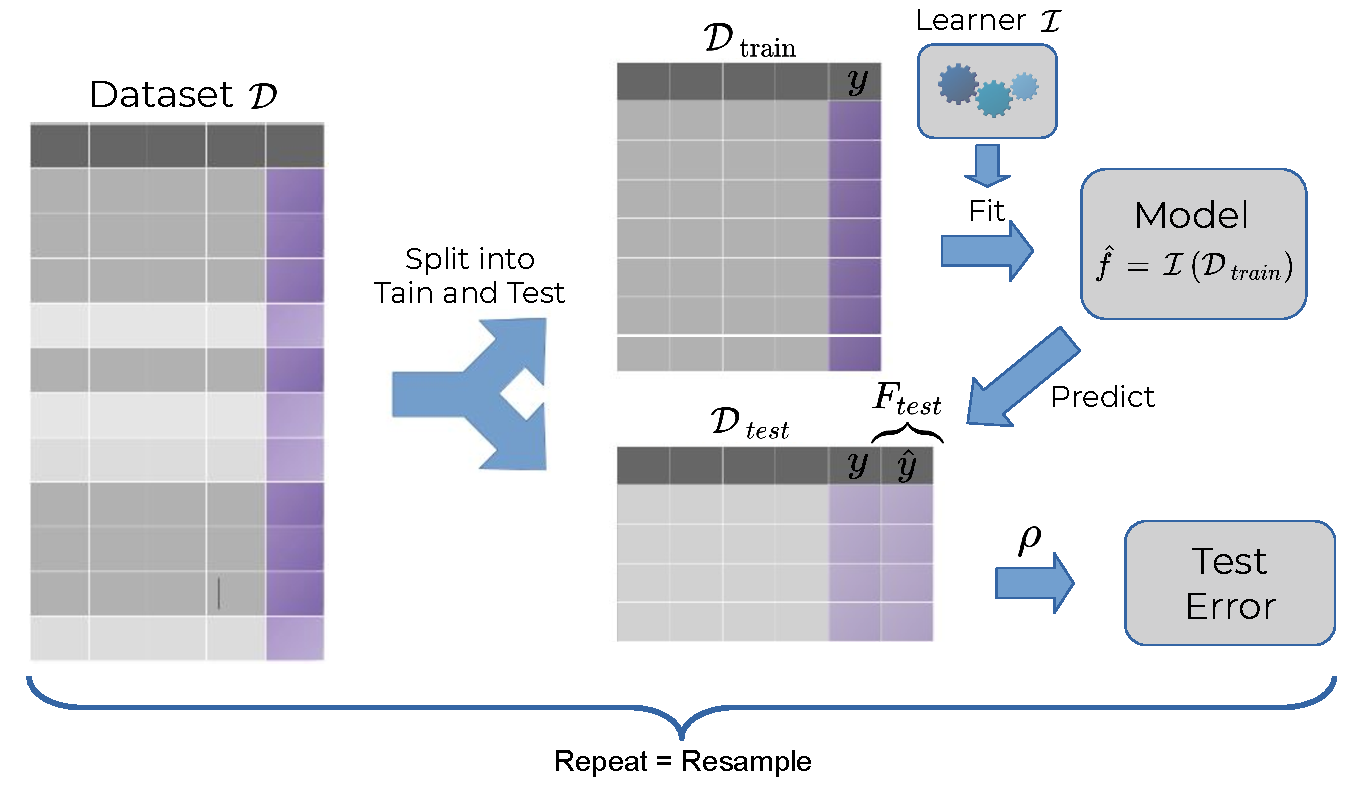
\includegraphics[width=0.6\textwidth]{figure_man/resampling_error.pdf}
% % FIGURE SOURCE: No source
% \includegraphics[width=0.7\textwidth]{figure_man/ml_abstraction-crop.pdf}
\end{center}

\end{vbframe}

% ------------------------------------------------------------------------------

\begin{vbframe}{Resampling strategies}

\begin{itemize}
  \item Different \textbf{resampling strategies} exist to balance bias against 
  variance, e.g., holdout sampling or cross-validation.
  \item To ease notation, we represent our train and test sets by index
  vectors $J_\mathrm{train} \in \nset^{m_\mathrm{train}}$ and $J_\mathrm{test}
  \in \nset^{m_\mathrm{test}}$, and define a resampling strategy with 
  $B$ train-test splits by $$\mathcal{J} = \left((J_{\mathrm{train}, 1}, 
  J_{\mathrm{test}, 1}), \dots, (J_{\mathrm{train}, B}, J_{\mathrm{test}, B}) 
  \right).$$
  % \item With this, we can denote the corresponding vector of labels as
  % $\yv_J = \left(y^{(J^{(1)})},\dots, y^{(J^{(m)})} \right) \in \Yspace^m$ and
  % the matrix of prediction scores as
  % $\bm{F}_{J,f} = \left( f(\xv^{(J^{(1)})}), \dots, f(\xv^{(J^{(m)})}) \right)
  % \in \R^{m\times g}$.
  % TODO translate to latex-math once notation is updated there
  \item Based on $\mathcal{J}$, we can express our \textbf{generalization error} 
  estimate for arbitrary resampling strategies as
  \begin{equation*}
    \begin{split}
      \small
      \widehat{\mathrm{GE}}_\mathcal{J}(\inducer, \lambdav, \rho) =
      \textrm{agg} \Bigg(& \rho \left( \yv_{J_{\mathrm{test}, 1}},
      \bm{F}_{J_{\mathrm{test}, 1}, \inducer(J_{\mathrm{test}, 1}, \lambdav)} 
      \right), \\
      &\dots, 
      \rho \left( \yv_{J_{\mathrm{test}, B}},
      \bm{F}_{J_{\mathrm{test}, B}, \inducer(J_{\mathrm{test}, B}, \lambdav)}
      \right) \Bigg),
    \end{split}
  \end{equation*}
  where the aggregation \textcolor{blue}{$\textrm{agg}$} is typically chosen to 
  be the mean.
\end{itemize}

\end{vbframe}

% ------------------------------------------------------------------------------

\begin{vbframe}{Cross-Validation}

\begin{itemize}
  \item Split the data into $k$ roughly equally-sized partitions.
  \item Use each part once as test set and join the respective $k-1$ others for 
  training.
  \item Obtain $k$ test errors and average.
\end{itemize}

\lz

\textbf{Example:} 3-fold cross-validation

\begin{center}
% FIGURE SOURCE: https://docs.google.com/presentation/d/1sKtnj5nIQrcOGU7rTisMsppUGOk7UX2gbjKhtQmTX7g/edit?usp=sharing
\includegraphics[width=8cm]{figure_man/crossvalidation.png}
\end{center}
\end{vbframe}

\begin{vbframe}{Cross-Validation - Stratification}

Stratification attempts to preserve the distribution of the target class (or any 
specific categorical feature of interest) in each fold.

\lz

\textbf{Example:} stratified 3-fold cross-validation

\lz

\begin{knitrout}\scriptsize
\definecolor{shadecolor}{rgb}{0.969, 0.969, 0.969}\color{fgcolor}

{\centering \includegraphics[width=0.95\textwidth]{figure/eval_resample_1} 

}

\end{knitrout}
\end{vbframe}

% ------------------------------------------------------------------------------

\begin{vbframe}{Cross-Validation}

\begin{itemize}
  \item 5 or 10 folds are common.%, they use 80\% and 90\% of data in training
  \item $k = n$ is known as leave-one-out (LOO) cross-validation.
  \item GE estimates tend to be pessimistically biased: 
  size of the training sets is $ n- \tfrac{n}{k} < n$. \\
  $\Rightarrow$ Bias increases as $k$ gets smaller.
  \item The $k$ performance estimates are dependent because
  of the structured overlap of the training sets.\\
  $\Rightarrow$ Variance of the estimator increases for very large $k$ 
  (approaching LOO), when training sets nearly completely overlap.
  % \item LOO is nearly unbiased, but has high variance.
  \item Repeated $k$-fold CV (multiple random partitions)
  can improve error estimation for small sample sizes.
\end{itemize}
\end{vbframe}

% ------------------------------------------------------------------------------

\begin{vbframe}{Bootstrap}

The basic idea is to randomly draw $B$ training sets of size $n$ with
replacement from the original training set $\Dtrain$:
% \begin{eqnarray*}
% \Dtrain^1 &=& \{z^1_1, \ldots, z^1_n\}\\
% \vdots& \\
% \Dtrain^B &=& \{z^B_1, \ldots, z^B_n\}
% \end{eqnarray*}

\begin{center}
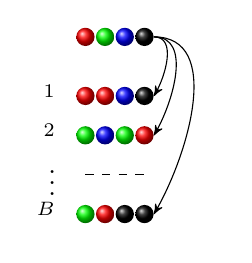
\begin{tikzpicture}[scale=1]
% style
\tikzstyle{rboule} = [circle,scale=0.7,ball color=red]
\tikzstyle{gboule} = [circle,scale=0.7,ball color=green]
\tikzstyle{bboule} = [circle,scale=0.7,ball color=blue]
\tikzstyle{nboule} = [circle,scale=0.7,ball color=black]
\tikzstyle{sample} = [->,thin]

% title initial sample
\path (3.5,3.75) node[anchor=east] {$\Dtrain$};

% labels
\path (3.5,3)   node[anchor=east] {$\Dtrain^1$};
\path (3.5,2.5) node[anchor=east] {$\Dtrain^2$};
\path (3.5,1.5) node[anchor=east] {$\Dtrain^B$};

\path (3.5,2) node[anchor=east] {$\vdots$};
\path[draw,dashed] (3.75,2.0) -- (4.5,2.0);

% initial sample
\path ( 3.75,3.75) node[rboule] (j01) {};
\path ( 4.00,3.75) node[gboule] (j02) {};
\path ( 4.25,3.75) node[bboule] (j03) {};
\path ( 4.5,3.75) node[nboule] (j20) {};

% bootstrap 1
\path ( 3.75, 3.0) node[rboule] {};
\path ( 4.00, 3.0) node[rboule] {};
\path ( 4.25, 3.0) node[bboule] {};
\path ( 4.5, 3.0) node[nboule] (b1) {};

% bootstrap 2
\path ( 3.75, 2.5) node[gboule] {};
\path ( 4.00, 2.5) node[bboule] {};
\path ( 4.25, 2.5) node[gboule] {};
\path ( 4.5, 2.5) node[rboule] (b2) {};

% bootstrap N
\path (3.75,1.5) node[gboule] {};
\path (4,1.5) node[rboule] {};
\path (4.25,1.5) node[nboule] {};
\path (4.5,1.5) node[nboule] (bN) {};

% arrows
\path[sample] (j20.east) edge [out=0, in=60] (b1.east);
\path[sample] (j20.east) edge [out=0, in=60] (b2.east);
\path[sample] (j20.east) edge [out=0, in=60] (bN.east);
\end{tikzpicture}
\end{center}

We define the test set in terms of out-of-bag observations
$\Dtest^b = \Dtrain \setminus \Dtrain^b$, $b = 1, 2, \dots, B$.

\framebreak

\begin{itemize}
  \item Typically, $B$ is between $30$ and $200$.
  \item The variance of the bootstrap estimator tends to be smaller than the
  variance of $k$-fold CV. \\
  $\Rightarrow$ More iterations, smaller variance.
  \item As in $k$-fold CV, GE estimates tend to be pessimistically biased
  (because training sets contain only about $63.2 \%$ of the unique 
  observations).
  \item Bootstrapping framework allows for inference 
  (e.g., detecting significant performance differences between learners).
  \item Extensions exist for very small data sets that also use the training 
  error for  estimation: B632 and B632+.
\end{itemize}

\end{vbframe}

% ------------------------------------------------------------------------------

\begin{vbframe}{Subsampling}

\begin{itemize}
  \item Repeated hold-out with averaging, a.k.a. Monte Carlo CV.
  \item Similar to bootstrap, but draws without replacement.
  \item Typical choices for splitting: $\frac{4}{5}$ or $\frac{9}{10}$ for 
  training.
\end{itemize}
\begin{center}
% FIGURE SOURCE: https://docs.google.com/drawings/d/1q7WN1_YKHedIPNySiZBEraLtTkHRX12Ej6M6ISbfMD0/edit?usp=sharing
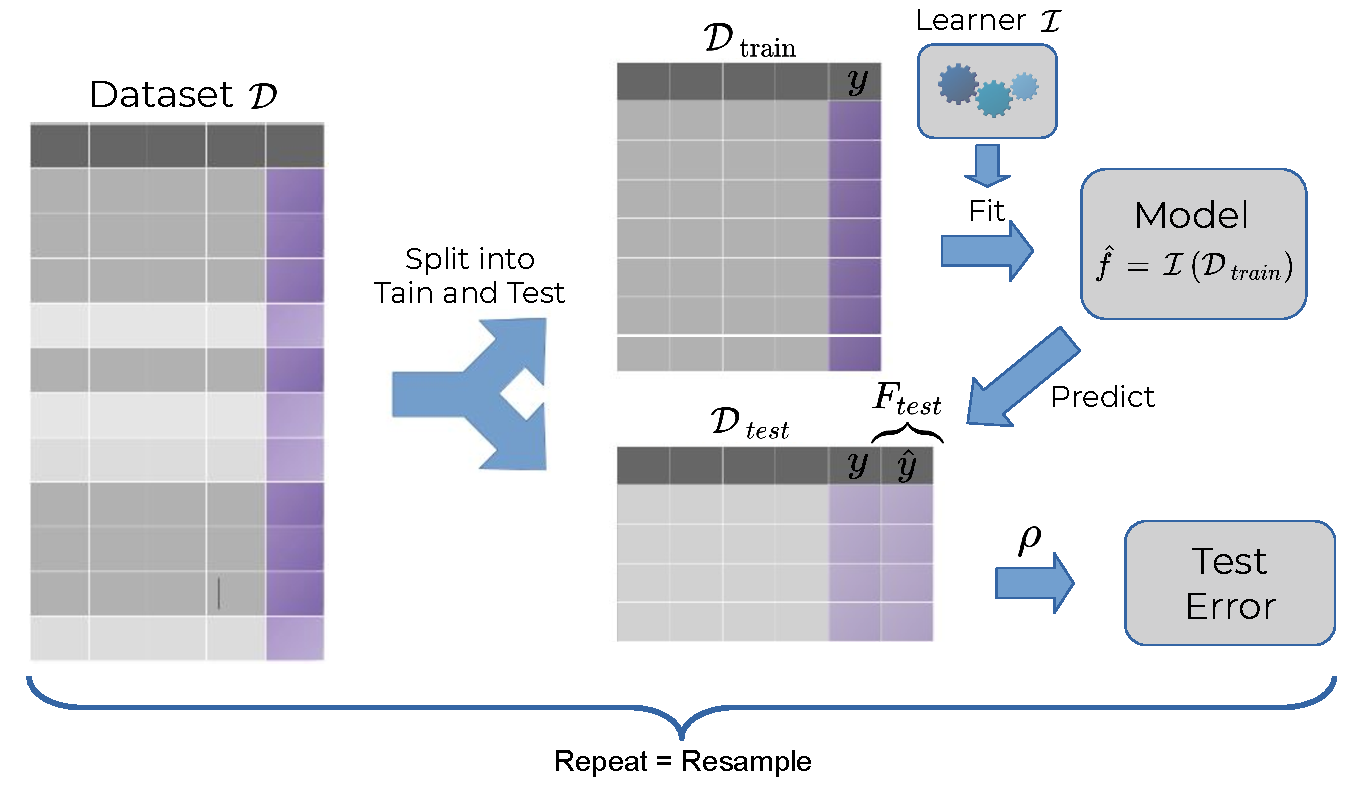
\includegraphics[width=0.7\textwidth]{figure_man/resampling_error.pdf}
\end{center}
\begin{itemize}
  \item The smaller the subsampling rate, the larger the pessimistic bias.
  \item The more subsampling repetitions, the smaller the variance.
\end{itemize}

\end{vbframe}

% ------------------------------------------------------------------------------

\begin{vbframe}{Bias-Variance Analysis for Subsampling}

  \begin{itemize}
    \item Reconsider our hold-out experiment on the \texttt{spirals} data from 
    the train-test unit (maybe re-read it again)
    \item Again, we use split rates $s \in \{0.05, 0.1, ..., 0.95\}$ for 
    training with $|\Dtrain| = s \cdot 500$.
    \item But: now we compare 50 subsampling experiments with $50 \cdot 50$ 
    hold-out experiments per split.
    \item Every subsampling experiment is the result of averaging 50 hold-out 
    experiments, so each performance estimate is much more reliable (but also 
    more expensive) than one computed by a single hold-out experiment.
  \end{itemize}

\framebreak

\begin{center}
% FIGURE SOURCE: eval-resampling-example
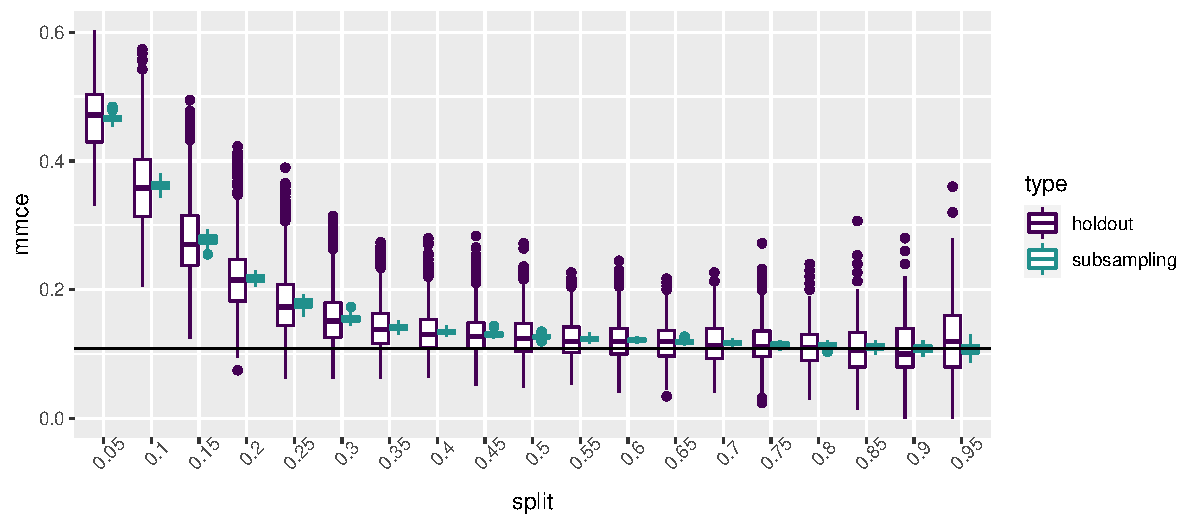
\includegraphics[width=0.9\textwidth]{figure/eval-resampling-example-1}
\end{center}



\begin{itemize}
  \item Both experiments are compared to the "real" MMCE (black line).
  \item Subsampling has the same pessimistic bias for small split rates but 
  much less variance overall.
  \item This allows to use much smaller test sets with good results.
\end{itemize}

\framebreak

\begin{center}
% FIGURE SOURCE: eval-resampling-example
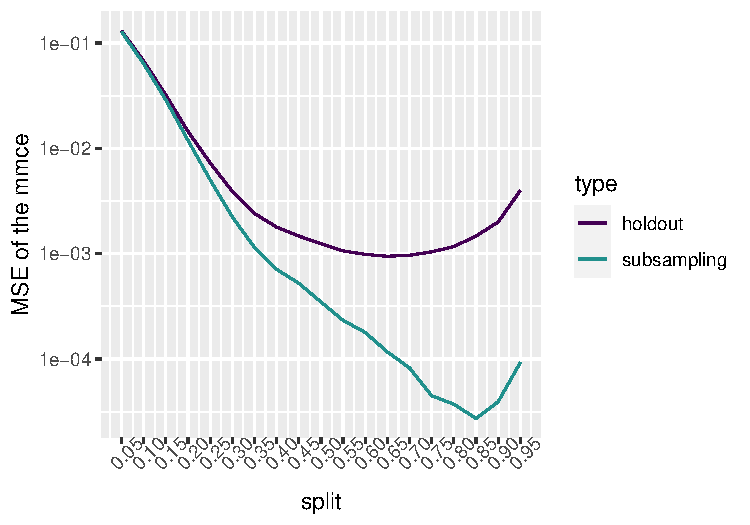
\includegraphics[width=0.7\textwidth]{figure/eval-resampling-example-2}
\end{center}

\begin{itemize}
  \item The MSE is strictly better for subsampling compared to hold-out.
  \item The optimal split rate now is a higher $s \approx 0.8$.
  \item We see the variance picking up at the end because training sets 
  increasingly overlap.
\end{itemize}

\end{vbframe}

% ------------------------------------------------------------------------------

\begin{vbframe}{Resampling discussion}

\begin{itemize}

  \item In ML we fit, at the end, a model on all our given data.\\

  \item \textbf{Problem:} We need to know how well this model will perform in 
  the future, but no data is left to reliably quantify this.\\
  $\Rightarrow$ Approximate using hold-out / CV / bootstrap / subsampling \\
  estimate\\ 

  \item \textbf{But:} pessimistic bias because we don't use all data points.\\

  \item The final model is (usually) computed on all data points.

  \item Strictly speaking, resampling only produces one number, the performance 
  estimator.
  It does NOT produce models, parameters, etc. These are intermediate results 
  and discarded.
  
  \item The model and parameters are only obtained when we finally fit the 
  learner on the complete data.

\end{itemize}

\framebreak

\begin{itemize}
  \item 5-CV or 10-CV have become standard.
  \item Do not use hold-out, CV with few iterations, or subsampling with a low 
  subsampling rate for small samples, since this can cause the estimator to be 
  extremely biased, with large variance.
  \item For small-data situations with less than 500 or 200 observations, use 
  LOO or, probably better, repeated CV.
  \item For some models, computationally fast calculations or approximations 
  for LOO exist.
  \item A data set $\D$ with $|\D| = 100.000$ can have small-sample properties 
  if one class has few observations 
  \item Research indicates that subsampling has better properties than
    bootstrapping. The repeated observations can cause problems in training,
    especially in nested setups where the \enquote{training} set is split up again.
\end{itemize}
\end{vbframe}

\endlecture
\end{document}
